\section{Frequency-domain PINN for a moving load}\label{sec:vf-fdpinn}

\subsection*{Concept and purpose}

\citet{liang2024fdpinn} replace the time-domain moving-load equation of a simply supported beam by one ordinary differential equation per frequency. A physics-informed neural network (PINN) then has to represent the spectrum, which is smooth in space and sharply peaked in frequency near the first natural frequency, instead of the oscillating time-domain field whose fast free vibration a network of modest size fits badly. The same network, with the bending stiffness $EI$ promoted to a trainable scalar, solves the inverse problem of identifying $EI$ from one sensor. The study tests the forward and inverse results on three beams, and checks whether the 0--5~Hz band used by the method already limits the accuracy.

The network training is outside the two packages (it uses PyTorch). The packages supply the reference fields: \fea{} with a moving-load class (\texttt{MovingPointLoad}, Hermite consistent nodal forces at $x=vt$), a Newmark and a modal-superposition solution, and the frequency-domain ROM of \rom{} for the band-truncation study.

\subsection*{Mathematics as implemented}

A simply supported Euler--Bernoulli beam under a load $p$ moving at speed $v$ obeys
\begin{equation}\label{eq:fd-pde}
EI\frac{\partial^4u}{\partial x^4}+c\frac{\partial u}{\partial t}+m\frac{\partial^2u}{\partial t^2}=p\,\delta(x-vt),\qquad t\in[0,L/v],
\end{equation}
with $u=u_{xx}=0$ at $x=0,L$ and the beam at rest at the start. The exact reference is modal superposition $u(x,t)=\sum_n\phi_n(x)q_n(t)$, $\phi_n=\sin(n\pi x/L)$; mode 1 dominates, with $f_1=3.5124$~Hz for the publication's beam.

\emph{Frequency-domain transform.} Transforming over one traversal, $\hat u(x,\omega)=\int_0^{L/v}u(x,t)e^{-i\omega t}\,dt$, turns \cref{eq:fd-pde} into an ordinary differential equation in $x$ for every $\omega$, because the Dirac load integrates in closed form:
\begin{equation}\label{eq:fd-fd}
EI\frac{\partial^4\hat u}{\partial x^4}+ic\omega\hat u-m\omega^2\hat u=\frac pve^{-ix\omega/v}.
\end{equation}
A network cannot output complex numbers, so $\hat u=\hat u_r+i\hat u_i$ is split into two real residuals,
\begin{equation}\label{eq:fd-split}
EI\,\hat u_{r,xxxx}-c\omega\hat u_i-m\omega^2\hat u_r=\tfrac pv\cos\tfrac{x\omega}v,\qquad
EI\,\hat u_{i,xxxx}+c\omega\hat u_r-m\omega^2\hat u_i=-\tfrac pv\sin\tfrac{x\omega}v,
\end{equation}
and the network maps $(x,\omega)$ to $(\hat u_r,\hat u_i)$. The displacement is recovered by the inverse transform over the band,
\begin{equation}\label{eq:fd-inv}
u(x,t)=\frac1{2\pi}\int_0^{\omega_{\max}}\hat u(x,\omega)e^{i\omega t}\,d\omega .
\end{equation}

\emph{Loss.} $\mathcal L=w_{DE}\mathcal L_{DE}+w_{BC}\mathcal L_{BC}+w_{ME}\mathcal L_{ME}$, where $\mathcal L_{DE}$ is the mean squared residual of \cref{eq:fd-split} at random $(x,\omega)$ collocation points (resampled every 100 iterations), $\mathcal L_{BC}$ enforces $\hat u=\hat u_{xx}=0$ at both ends, and $\mathcal L_{ME}$, used for the inverse problem only, is the misfit to the sensor spectrum at mid-span. Each weight is the reciprocal of its term's initial value.

\emph{Inverse problem.} $EI$ is a trainable scalar $\theta=EI/EI_{\rm true}$ multiplying only the fourth-derivative term, started at $EI_0=5\times10^9$. One sensor sits at $x=L/2$. The accuracy and the field error are
\begin{equation}\label{eq:fd-acc}
\mathrm{acc}=1-\frac{|EI_{\rm id}-EI_{\rm true}|}{EI_{\rm id}},\qquad\mathrm{nMSE}=\operatorname{mean}\big[(\tilde u-\tilde u_{\rm ref})^2\big],
\end{equation}
with the tilde denoting min--max normalisation. The accuracy divides by the identified $EI$, so an $EI$ that is $5.8\,\%$ high scores $94.56\,\%$ and not $94.2\,\%$.

\emph{Band truncation and resonance.} Restricting the spectrum to 0--5~Hz costs a quantifiable error, computed here from the frequency-domain solution; it is the error floor of any method that works in that band. The relation between stiffness and frequency, $f_1\propto\sqrt{EI}$, gives
\begin{equation}\label{eq:fd-f1}
\frac{\Delta f_1}{f_1}\approx\frac12\frac{\Delta EI}{EI}=2.8\,\%\ \text{ for }\ \frac{\Delta EI}{EI}=5.7\,\%,
\end{equation}
and the damping ratio $\xi=0.025$ gives the first mode a quality factor $Q=1/(2\xi)=20$ and a half-power width $\Delta f_{1/2}=2\xi f_1=0.176$~Hz, $3.5\,\%$ of the band.

\subsection*{Geometry and mesh}

The beam is the one of the publication, $L=20$~m with $EI=2.4\times10^9$~N\,m$^2$, $m=3000$~kg/m, a damping ratio of $0.025$ and a 12~kN load, in three cases that differ only in the load speed. The network has no mesh; its domain is the rectangle $(x,\omega)$ with random collocation points (\Cref{fig:vf-fd-geom}). The finite element references are the \fea{} Newmark and modal-superposition solutions; the report does not state their mesh.

\begin{figure}[tbp]
\centering
\includegraphics[width=0.98\linewidth]{figures/ch14_geom_fdpinn.pdf}
\caption{Moving-load beam of the study, drawn from the data of the report. (a) The simply supported beam, the load at $x=vt$ and the mid-span sensor of the inverse problem. (b) The domain of the network, $(x/L,\omega)$ with the 0--5~Hz band, and a random set of collocation points.}\label{fig:vf-fd-geom}
\end{figure}

\begin{table}[tbp]
\centering\footnotesize
\caption{The three cases ($f_1=3.512$~Hz in all).}\label{tab:vf-fd-cases}
\begin{tabular}{@{}rrrrrrrr@{}}
\toprule
Case & $v$ (m/s) & $L$ (m) & $EI$ (N m$^2$) & $m$ (kg/m) & Damping ratio & $p$ (kN) & Load frequency $v/2L$ (Hz)\\
\midrule
1 & 50 & 20 & $2.4\times10^9$ & 3000 & 0.025 & 12 & 1.25\\
2 & 20 & 20 & $2.4\times10^9$ & 3000 & 0.025 & 12 & 0.5\\
3 & 15 & 20 & $2.4\times10^9$ & 3000 & 0.025 & 12 & 0.375\\
\bottomrule
\end{tabular}
\end{table}

\begin{table}[tbp]
\centering\footnotesize
\caption{Set-up and deviations from the publication.}\label{tab:vf-fd-setup}
\begin{tabularx}{\linewidth}{@{}>{\raggedright\arraybackslash}p{3.0cm} >{\raggedright\arraybackslash}X >{\raggedright\arraybackslash}X@{}}
\toprule
Item & Publication & This work\\
\midrule
Network & $3\times60$, tanh, Glorot & same\\
Collocation points & 20\,000, resampled every 100 iterations & 5\,000, resampled every 100\\
Optimiser, budget & L-BFGS, $4\times10^5$ iterations ($10^4$ for the early comparison) & 1000 Adam + up to 15\,000 L-BFGS\\
Framework, hardware & DeepXDE, V100 32 GB & PyTorch, GTX 1050, single precision\\
Output scaling & an output transform & none (an amplitude envelope was tried and did not help)\\
Initial condition & $u=u_{tt}=0$ as written & $u=u_t=0$\\
Time-domain PINN & Gaussian Dirac, fixed $\sigma=0.1$ & source width ramped from $\sigma/L=0.1$ to $0.005$\\
Inverse sensor data & DFT of the sensor record (Eq.~19) & exact frequency-domain solution at $L/2$, 201 frequencies, no noise\\
Damping in the inverse problem & not stated & fixed at its true value; only $EI$ identified\\
Seeds & not stated & one per result\\
\bottomrule
\end{tabularx}
\end{table}

Two choices need explanation. The DFT of a finite record is inconsistent with the frequency-domain equation, because the beam keeps vibrating after $t=L/v$ while the transform assumes one stationary traversal, so the exact spectrum is used to avoid a data error that would bias $EI$; the publication may handle this differently. The source-width ramp was needed because with the plain recipe the time-domain PINN stayed at an nMSE of about $0.22$, a near-zero solution, in single and double precision; starting from a wide Gaussian and narrowing it was the only change that trained. Early stopping restores the best weights; for the inverse problem two rules were used, stopping on the accuracy against the true $EI$ (benchmark only, not usable in practice) and stopping on a fixed validation loss (needs no true $EI$), and each result below states which.

\subsection*{Results: reference solutions and band truncation}

The reference fields are exact: the analytical modal solution, a finite element Newmark integration and a finite element modal-superposition solution agree to about $10^{-7}$ or better in all six cases (Cases 1--3 and the appendix beams B1--B3), and the frequency-domain solution restricted to 0--5~Hz differs from the analytical one only by band-limiting (\Cref{fig:vf-fd-ref}). The band-limiting error is concentrated at the start and end of the traversal, where the load enters and leaves the beam and the response has broadband content, and it falls quickly with the band (\Cref{tab:vf-fd-band}, \Cref{fig:vf-fdpinn}a).

\begin{figure}[tbp]
\centering
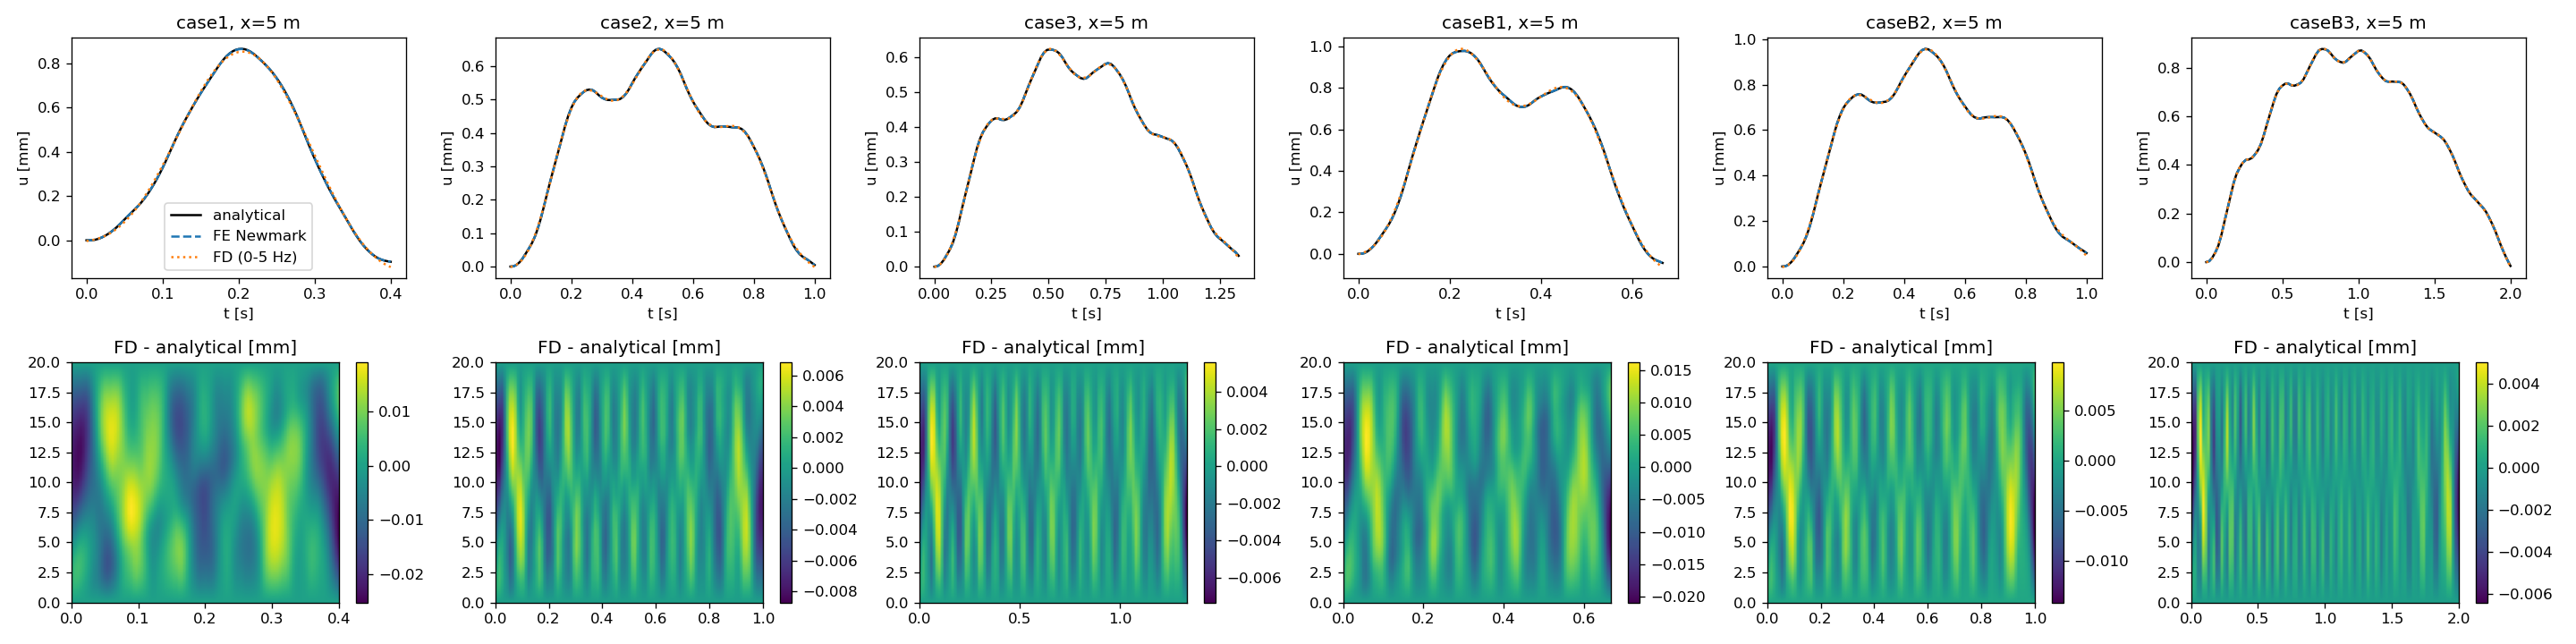
\includegraphics[width=0.9\linewidth]{figures/ch14r/fd_ref.png}
\caption{Reference solutions: analytical, finite element Newmark and the 0--5~Hz frequency-domain solution, and the band-limiting error field. Plot of the reproduction report.}\label{fig:vf-fd-ref}
\end{figure}

\begin{table}[tbp]
\centering\footnotesize
\caption{Normalised mean-square error of the band-limited solution against the analytical one.}\label{tab:vf-fd-band}
\begin{tabular}{@{}rrrrrr@{}}
\toprule
Case & 2.5 Hz & 5 Hz (publication) & 10 Hz & 20 Hz & Publication's FD-PINN MSE\\
\midrule
1 & $1.2\times10^{-2}$ & $3.8\times10^{-5}$ & $1.0\times10^{-5}$ & $2.7\times10^{-7}$ & $4.7\times10^{-5}$\\
2 & $2.5\times10^{-3}$ & $5.6\times10^{-6}$ & $2.3\times10^{-6}$ & $5.8\times10^{-8}$ & $7.2\times10^{-5}$\\
3 & $1.2\times10^{-3}$ & $4.0\times10^{-6}$ & $1.4\times10^{-6}$ & $3.3\times10^{-8}$ & $7.0\times10^{-5}$\\
\bottomrule
\end{tabular}
\end{table}

\begin{figure}[tbp]
\centering
\includegraphics[width=0.9\linewidth]{figures/ch14_fdpinn.pdf}
\caption{Moving-load beam of \citet{liang2024fdpinn}. (a) Normalised error of the band-limited field against the band width, full-order sweep; the cost of the 5~Hz band is \cvfFdBandOne, \cvfFdBandTwo{} and \cvfFdBandThree{} for the three cases. (b) The same error from frequency-domain ROMs of size $r$; with ten modes they agree with the full-order value to within \cvfFdTen. Redrawn by \texttt{scripts/ch14\_assets.py} from the saved outputs of the study; the study itself was not re-run for this book.}\label{fig:vf-fdpinn}
\end{figure}

For the comparison with the publication this matters as follows. In Case 1 the band alone accounts for $3.8\times10^{-5}$ of the publication's $4.7\times10^{-5}$ (about $80\,\%$), so its Case 1 result is close to the best any 0--5~Hz method can do; in Cases 2 and 3 the band accounts for only about $8\,\%$ and $6\,\%$ of its error, and the rest is network error, which is where this reproduction falls short.

\subsection*{Results: forward problem}

Only Case 3 was run forward. FD-PINN beats the time-domain PINN ($2.38\times10^{-3}$ against $3.90\times10^{-3}$) but not by the publication's margin: $7.0\times10^{-5}$ against $1.56\times10^{-3}$, a factor of 22, where this work obtains 1.6 (\Cref{tab:vf-fd-fwd}).

\begin{table}[tbp]
\centering\footnotesize
\caption{Forward problem, Case 3 (nMSE).}\label{tab:vf-fd-fwd}
\begin{tabular}{@{}lrrr@{}}
\toprule
Model & This work & Publication & Ratio\\
\midrule
Time-domain PINN & $3.90\times10^{-3}$ & $1.56\times10^{-3}$ & 2.5\\
FD-PINN & $2.38\times10^{-3}$ & $7.0\times10^{-5}$ & 34\\
\bottomrule
\end{tabular}
\end{table}

\emph{Time-domain PINN.} The plain recipe never left the near-zero solution; after the source Gaussian was widened and then narrowed during training, the best weights came at iteration 6000 when $\sigma/L$ had narrowed to about $0.019$. Without early stopping the error rose again to $0.027$. The result shows the spectral bias the publication describes: the network learns a smooth envelope and misses the 3.5~Hz oscillation (the double hump in the mid-span history), although the peak is close ($0.89$ against $0.87$~mm) (\Cref{fig:vf-fd-pinn}).

\emph{FD-PINN.} The nMSE stayed at $0.07$--$0.2$ for the first 7000 iterations, then fell to about $5\times10^{-3}$ at iteration 9000 and $2.4\times10^{-3}$ at 13\,000, where early stopping restored the weights. The error against the band-limited reference is $2.37\times10^{-3}$, so band truncation ($4\times10^{-6}$) is not the cause: the network under-fits the spectrum, reproducing the 0--1~Hz lobe but smoothing the small side lobes and the 3.5~Hz resonance peak, which is why the time history misses the double hump near $t=0.5$--$0.8$~s. The peak displacement is $0.869$ against $0.872$~mm (\Cref{fig:vf-fd-fdpinn}).

\begin{figure}[tbp]
\centering
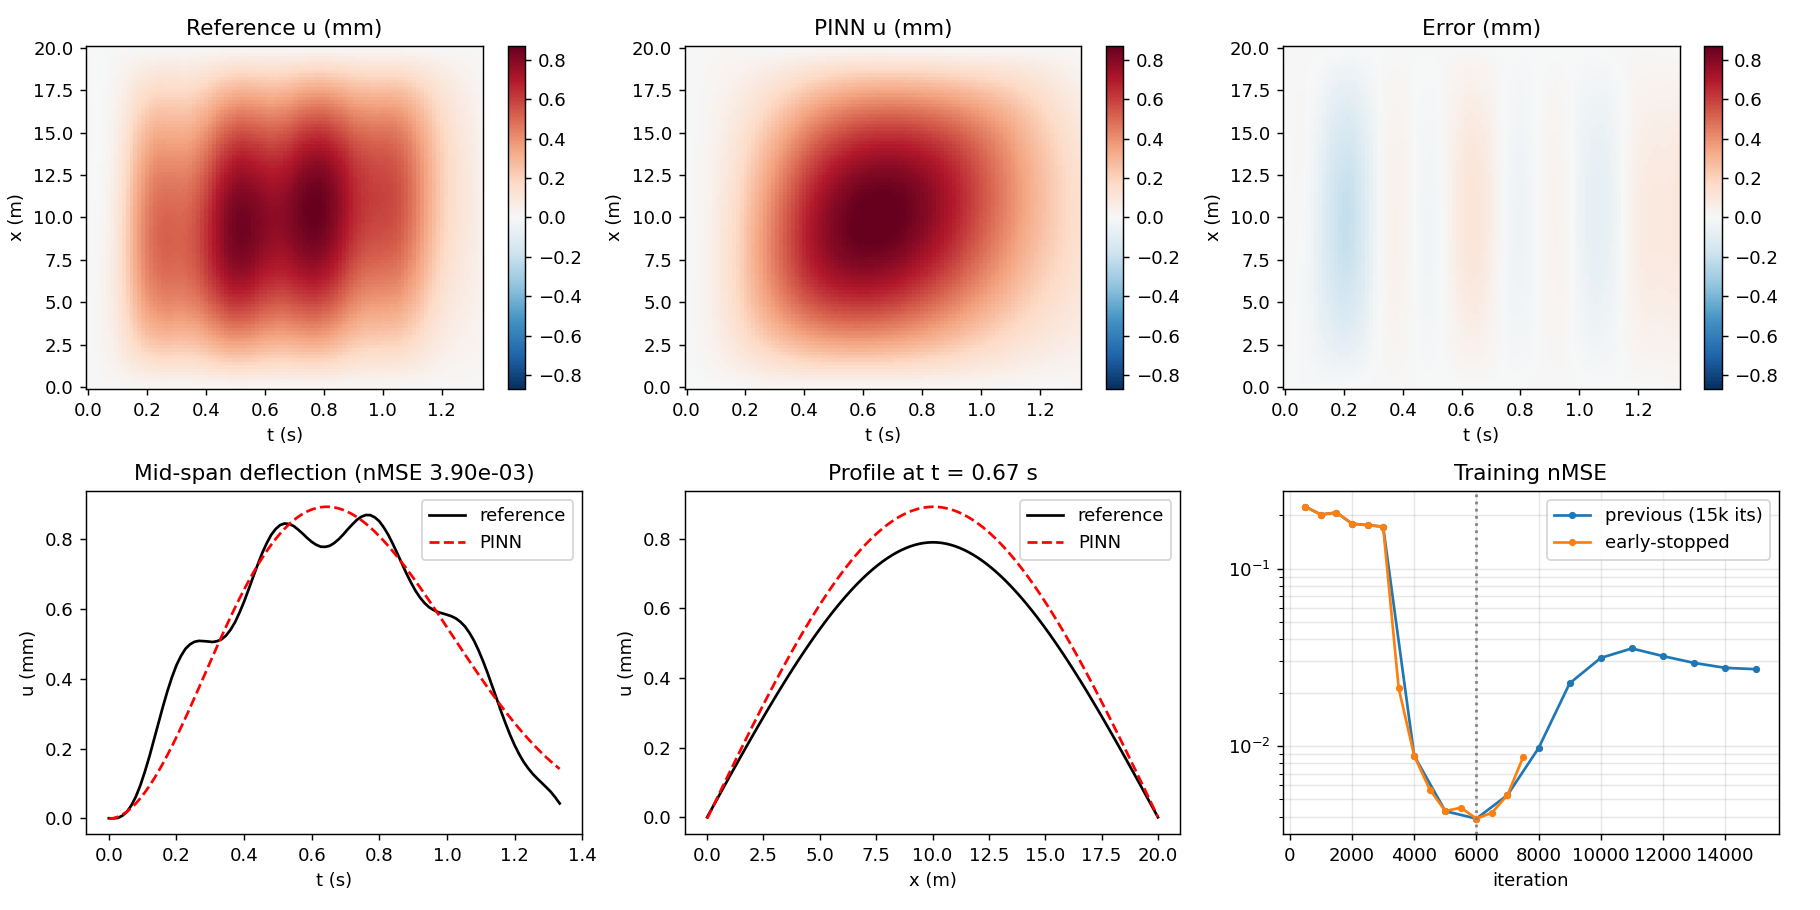
\includegraphics[width=0.95\linewidth]{figures/ch14r/fd_pinn.png}
\caption{Time-domain PINN, Case 3: fields, error, mid-span history, profile and training nMSE. Plot of the reproduction report.}\label{fig:vf-fd-pinn}
\end{figure}

\begin{figure}[tbp]
\centering
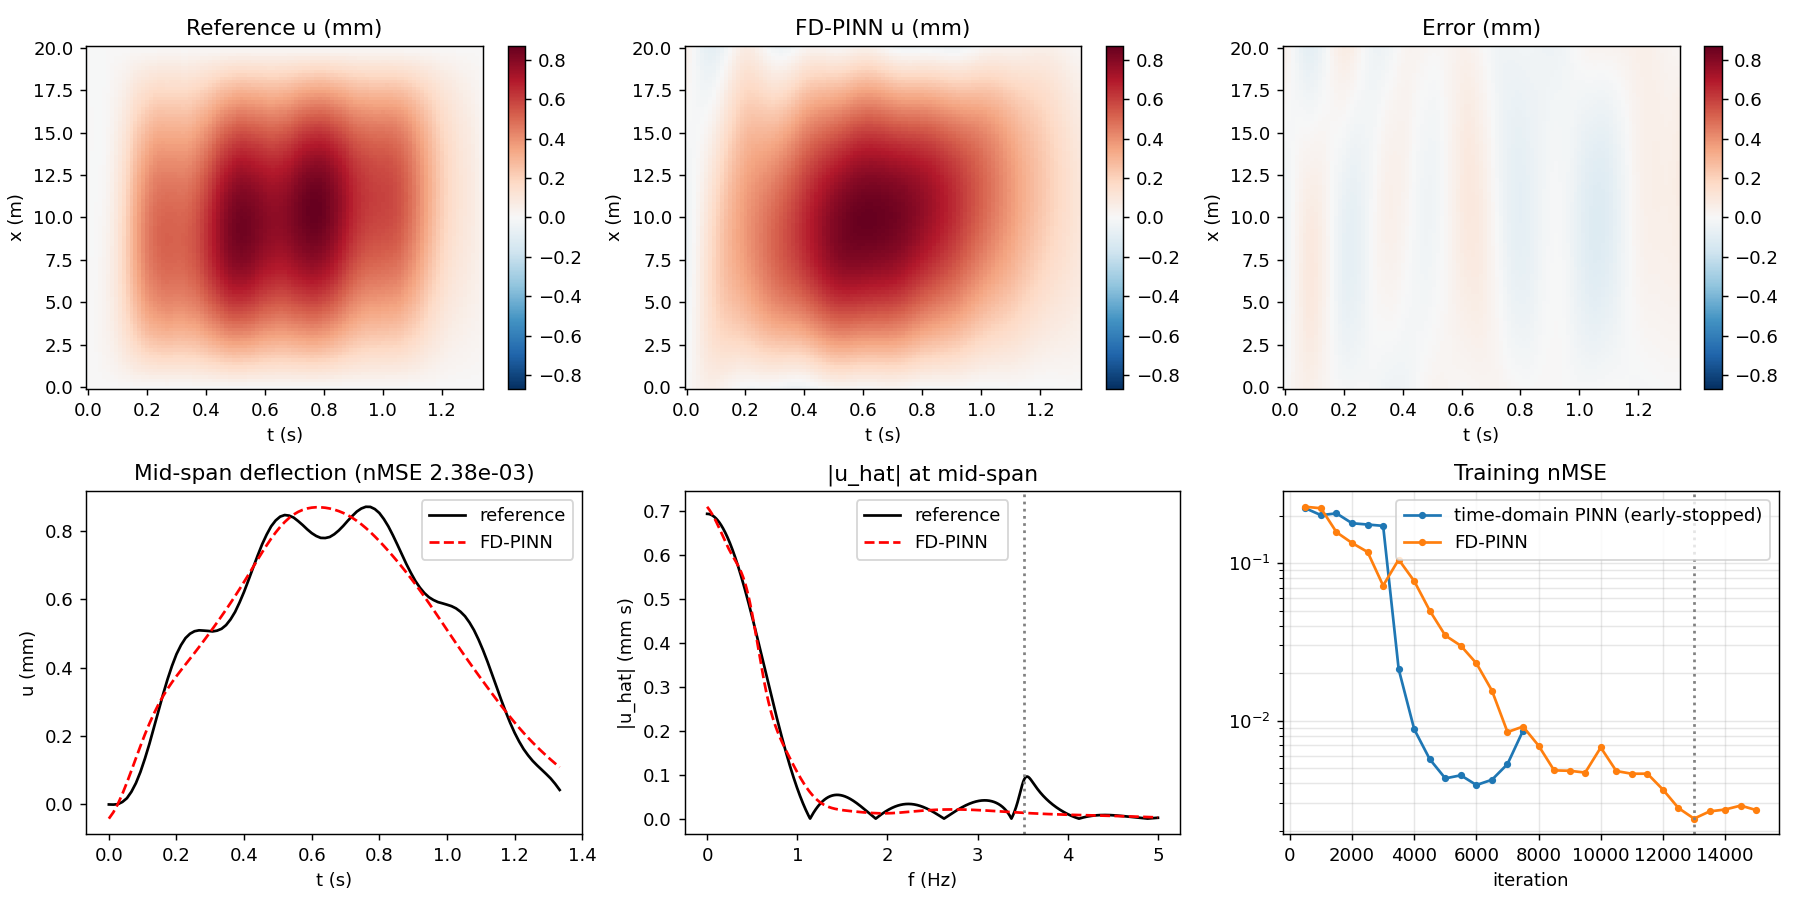
\includegraphics[width=0.95\linewidth]{figures/ch14r/fd_fdpinn.png}
\caption{FD-PINN, Case 3: fields, mid-span history, mid-span spectrum and training nMSE. Plot of the reproduction report.}\label{fig:vf-fd-fdpinn}
\end{figure}

\emph{Attempts to close the gap.} \Cref{tab:vf-fd-try} lists three changes, none of which helped; the 20\,000-point run converged much faster early (nMSE $8.3\times10^{-3}$ at iteration 4500 against $5.0\times10^{-2}$) but plateaued, and a patience of four stopped it. The baseline had the same plateau before dropping at iteration 12\,000, so the comparison is inconclusive (\Cref{fig:vf-fd-cmp}).

\begin{table}[tbp]
\centering\footnotesize
\caption{Changes tried on the forward FD-PINN, Case 3.}\label{tab:vf-fd-try}
\begin{tabularx}{\linewidth}{@{}>{\raggedright\arraybackslash}p{5.2cm} >{\raggedright\arraybackslash}X >{\raggedright\arraybackslash}p{3.0cm}@{}}
\toprule
Change & Result & Outcome\\
\midrule
Frequency-normalised residual (divide by the mode-1 operator) & nMSE $0.24$ at iteration 3000 against $0.072$ baseline & worse; NaN restarts\\
Mode-1 amplitude envelope on the output & faster start, then stalled at $0.087$ & worse than baseline\\
20\,000 collocation points & $4.48\times10^{-3}$, stopped at iteration 8000 & not better; early stop may be premature\\
\bottomrule
\end{tabularx}
\end{table}

\begin{figure}[tbp]
\centering
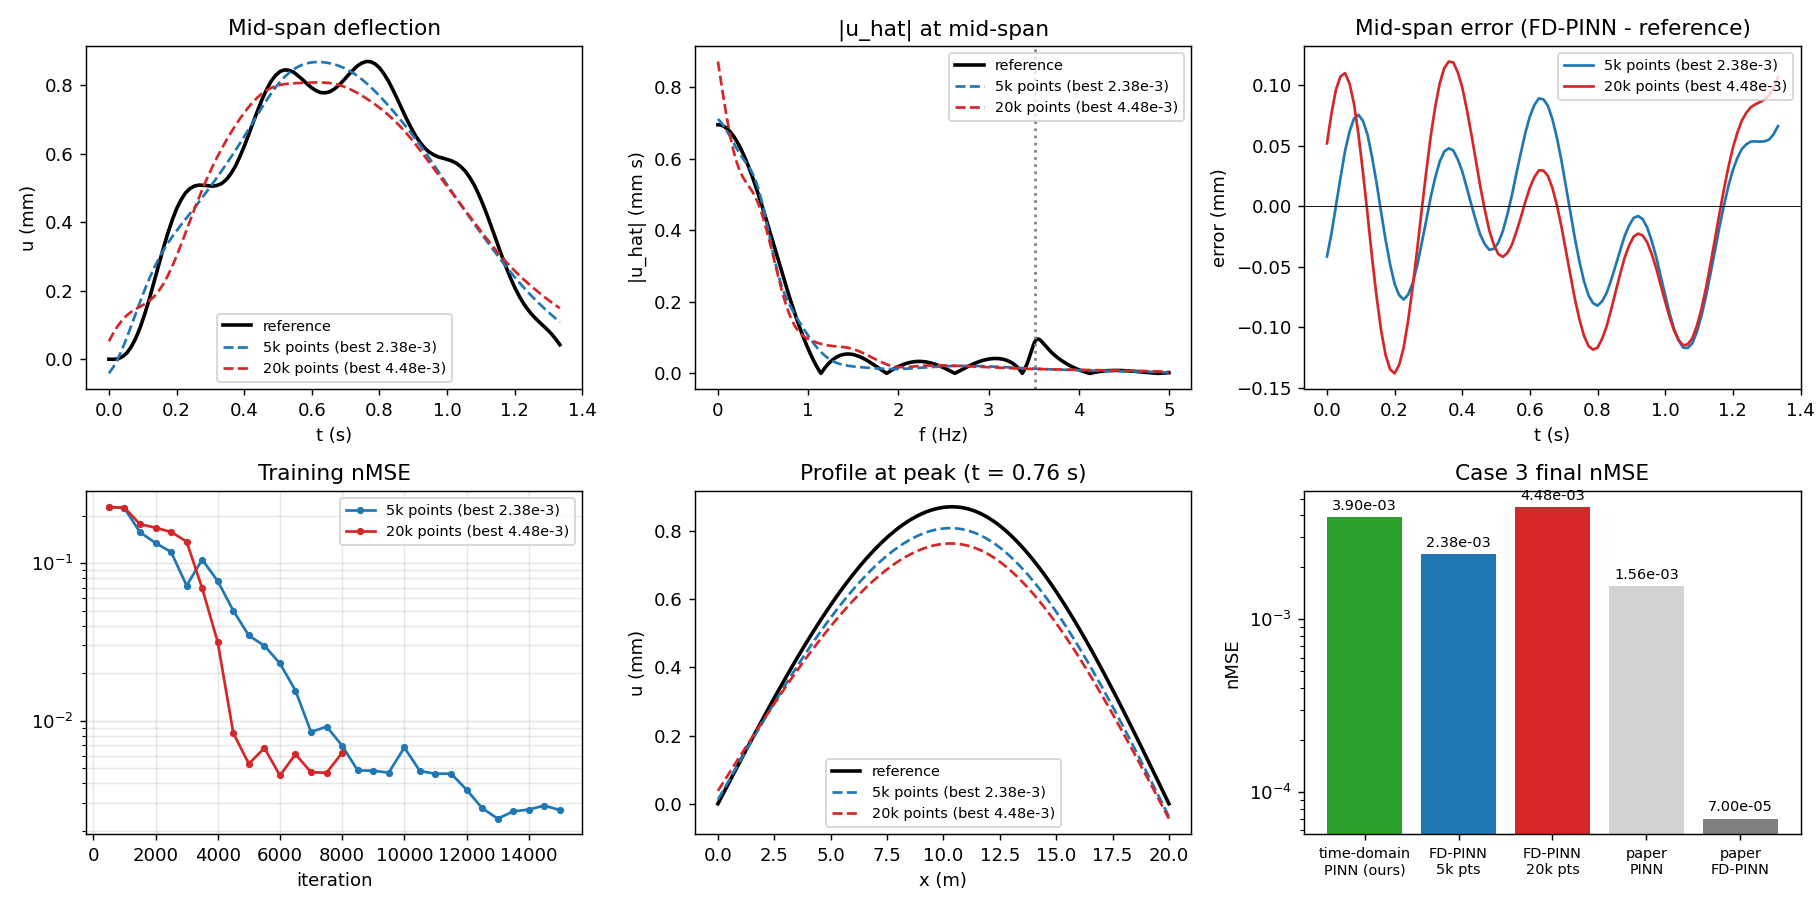
\includegraphics[width=0.95\linewidth]{figures/ch14r/fd_cmp.png}
\caption{FD-PINN with 5000 and 20\,000 collocation points: mid-span history, spectrum, profile and training nMSE. Plot of the reproduction report.}\label{fig:vf-fd-cmp}
\end{figure}

\subsection*{Results: inverse problem}

At the publication's $10^4$-iteration budget the identification accuracy matches or exceeds the publication in all three cases (\Cref{tab:vf-fd-inv}), but its near $100\,\%$ at $4\times10^5$ iterations is not reached, and the field error is three times higher in Case 2 and fifteen times higher in Case 3 (Case 1 is below the publication's). The rule that picks the reported iteration matters: stopping on the true $EI$ is a benchmark-only shortcut that picked the moments when the $EI$ trace crossed $2.4\times10^9$ (Case 3 reached $97.6\,\%$ at iteration 5000, Case 2 $98.9\,\%$ at iteration 2000 with a field nMSE of $2.9\times10^{-3}$), which are not converged values; the loss-rule rows are the fair ones. For Case 1 the $EI$ sat within $0.1\,\%$ for thousands of iterations, so both rules agree.

\begin{table}[tbp]
\centering\footnotesize
\setlength{\tabcolsep}{4pt}
\caption{Inverse identification of $EI$.}\label{tab:vf-fd-inv}
\begin{tabular}{@{}lrrrrrr@{}}
\toprule
Case & $EI$ identified & Accuracy (this work) & Publication, $10^4$ its & Publication, $4\times10^5$ its & Field nMSE (this work) & Publication MSE\\
\midrule
1 (true-$EI$ rule) & $2.3999\times10^9$ & $100.0\,\%$ & $99.6\,\%$ & $100\,\%$ & $3.75\times10^{-5}$ & $4.72\times10^{-5}$\\
2 (loss rule) & $2.4264\times10^9$ & $98.9\,\%$ & $95.8\,\%$ & $100\,\%$ & $2.31\times10^{-4}$ & $7.15\times10^{-5}$\\
3 (loss rule) & $2.5382\times10^9$ & $94.6\,\%$ & $94.4\,\%$ & $100\,\%$ & $1.08\times10^{-3}$ & $7.01\times10^{-5}$\\
\bottomrule
\end{tabular}
\end{table}

Case 1 converges cleanly ($EI$ within $0.1\,\%$ from iteration 2000). Case 2 needed about 7500 iterations: $EI$ sat near $2.6\times10^9$ until iteration 4500 and then settled within $1$--$1.7\,\%$ of $2.4\times10^9$. Case 3 settles $5.7$--$6\,\%$ high from iteration 3000 while the loss keeps falling (\Cref{fig:vf-fd-train,fig:vf-fd-fields}). All runs use one seed, and the $5\,\%$-improvement stopping rule is weak: in both loss-rule runs many small drops of $2$--$3\,\%$ per evaluation kept resetting the patience counter, so the runs used the full 16\,000 iterations.

\begin{figure}[tbp]
\centering
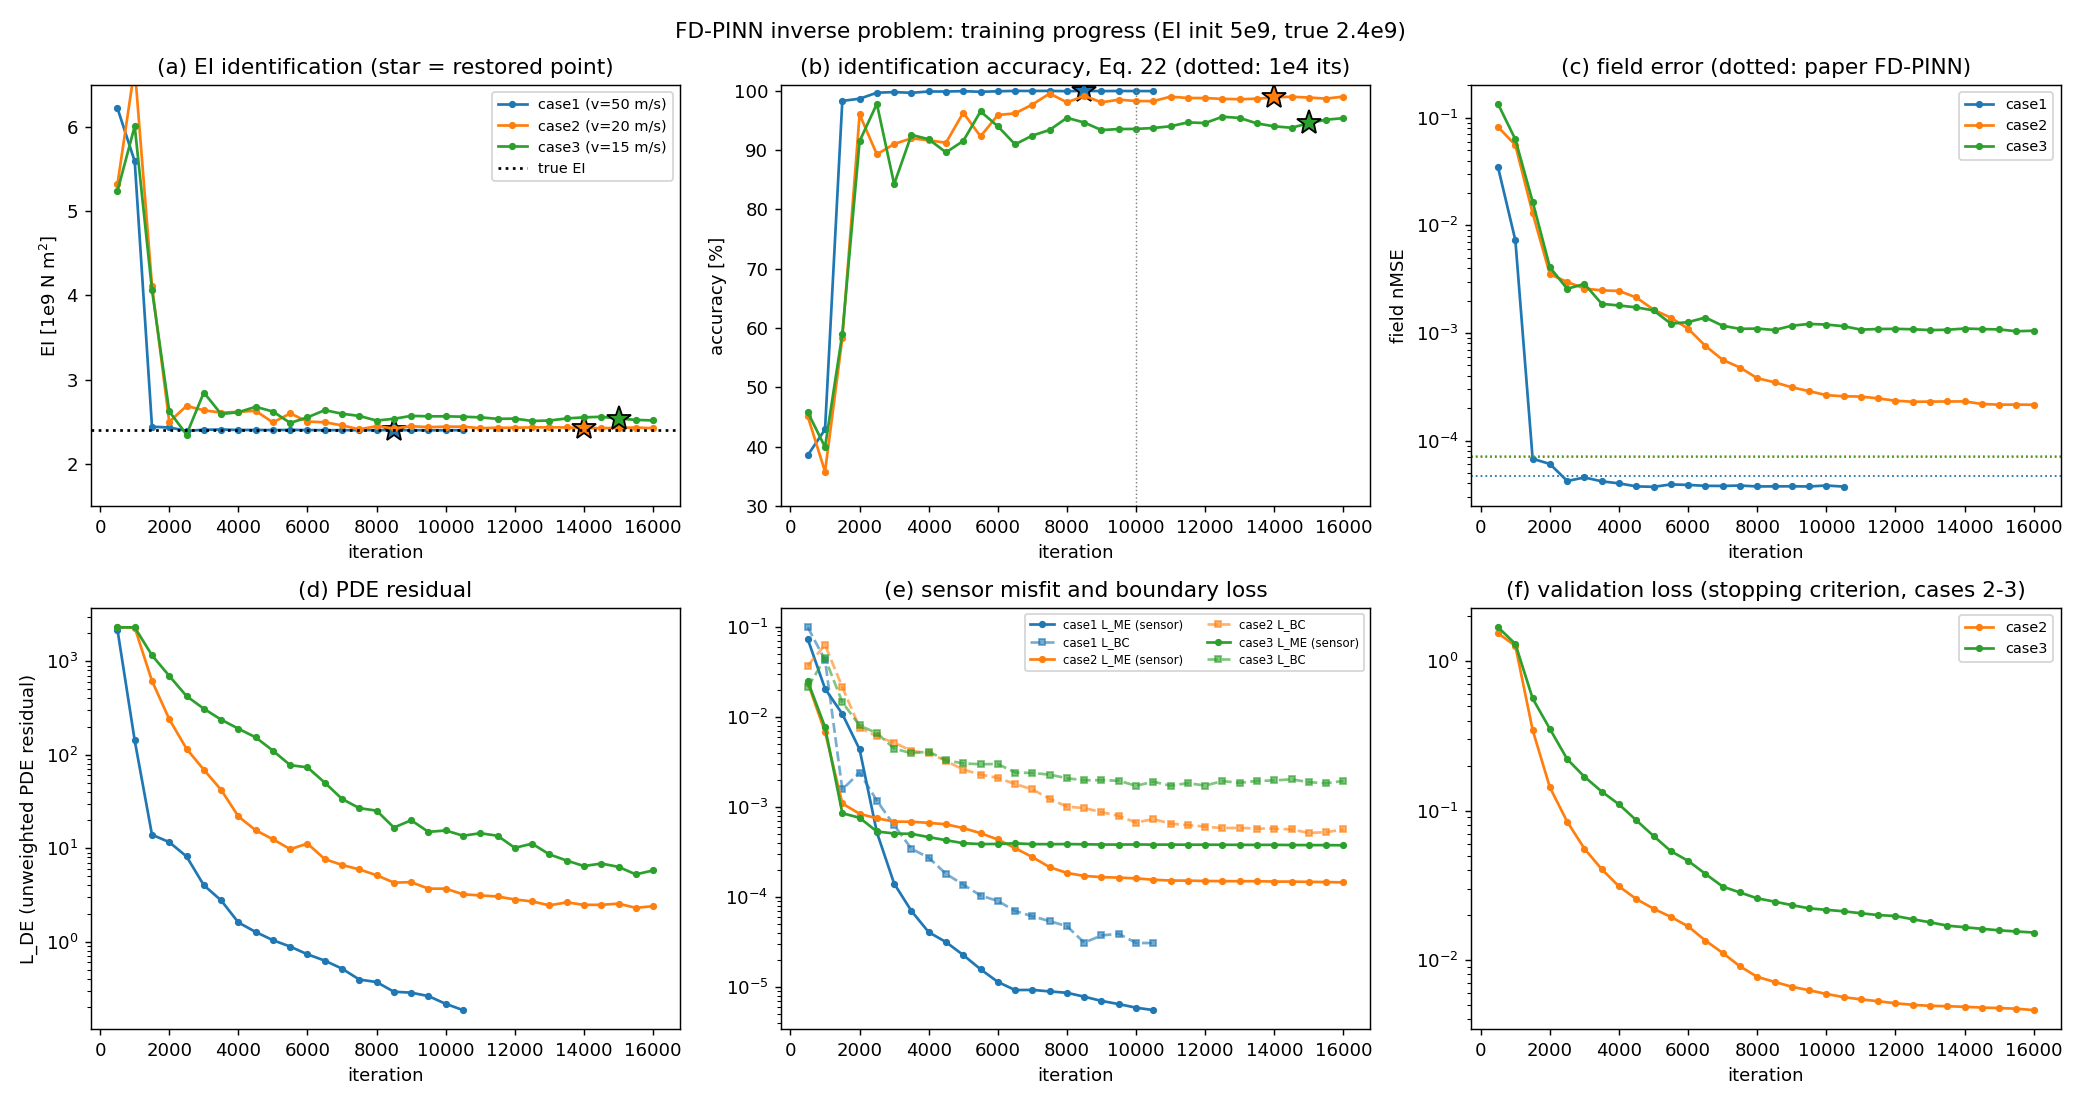
\includegraphics[width=0.95\linewidth]{figures/ch14r/fd_inv_train.png}
\caption{Inverse training: $EI$, accuracy and loss terms against iteration, three cases. Plot of the reproduction report.}\label{fig:vf-fd-train}
\end{figure}

\begin{figure}[tbp]
\centering
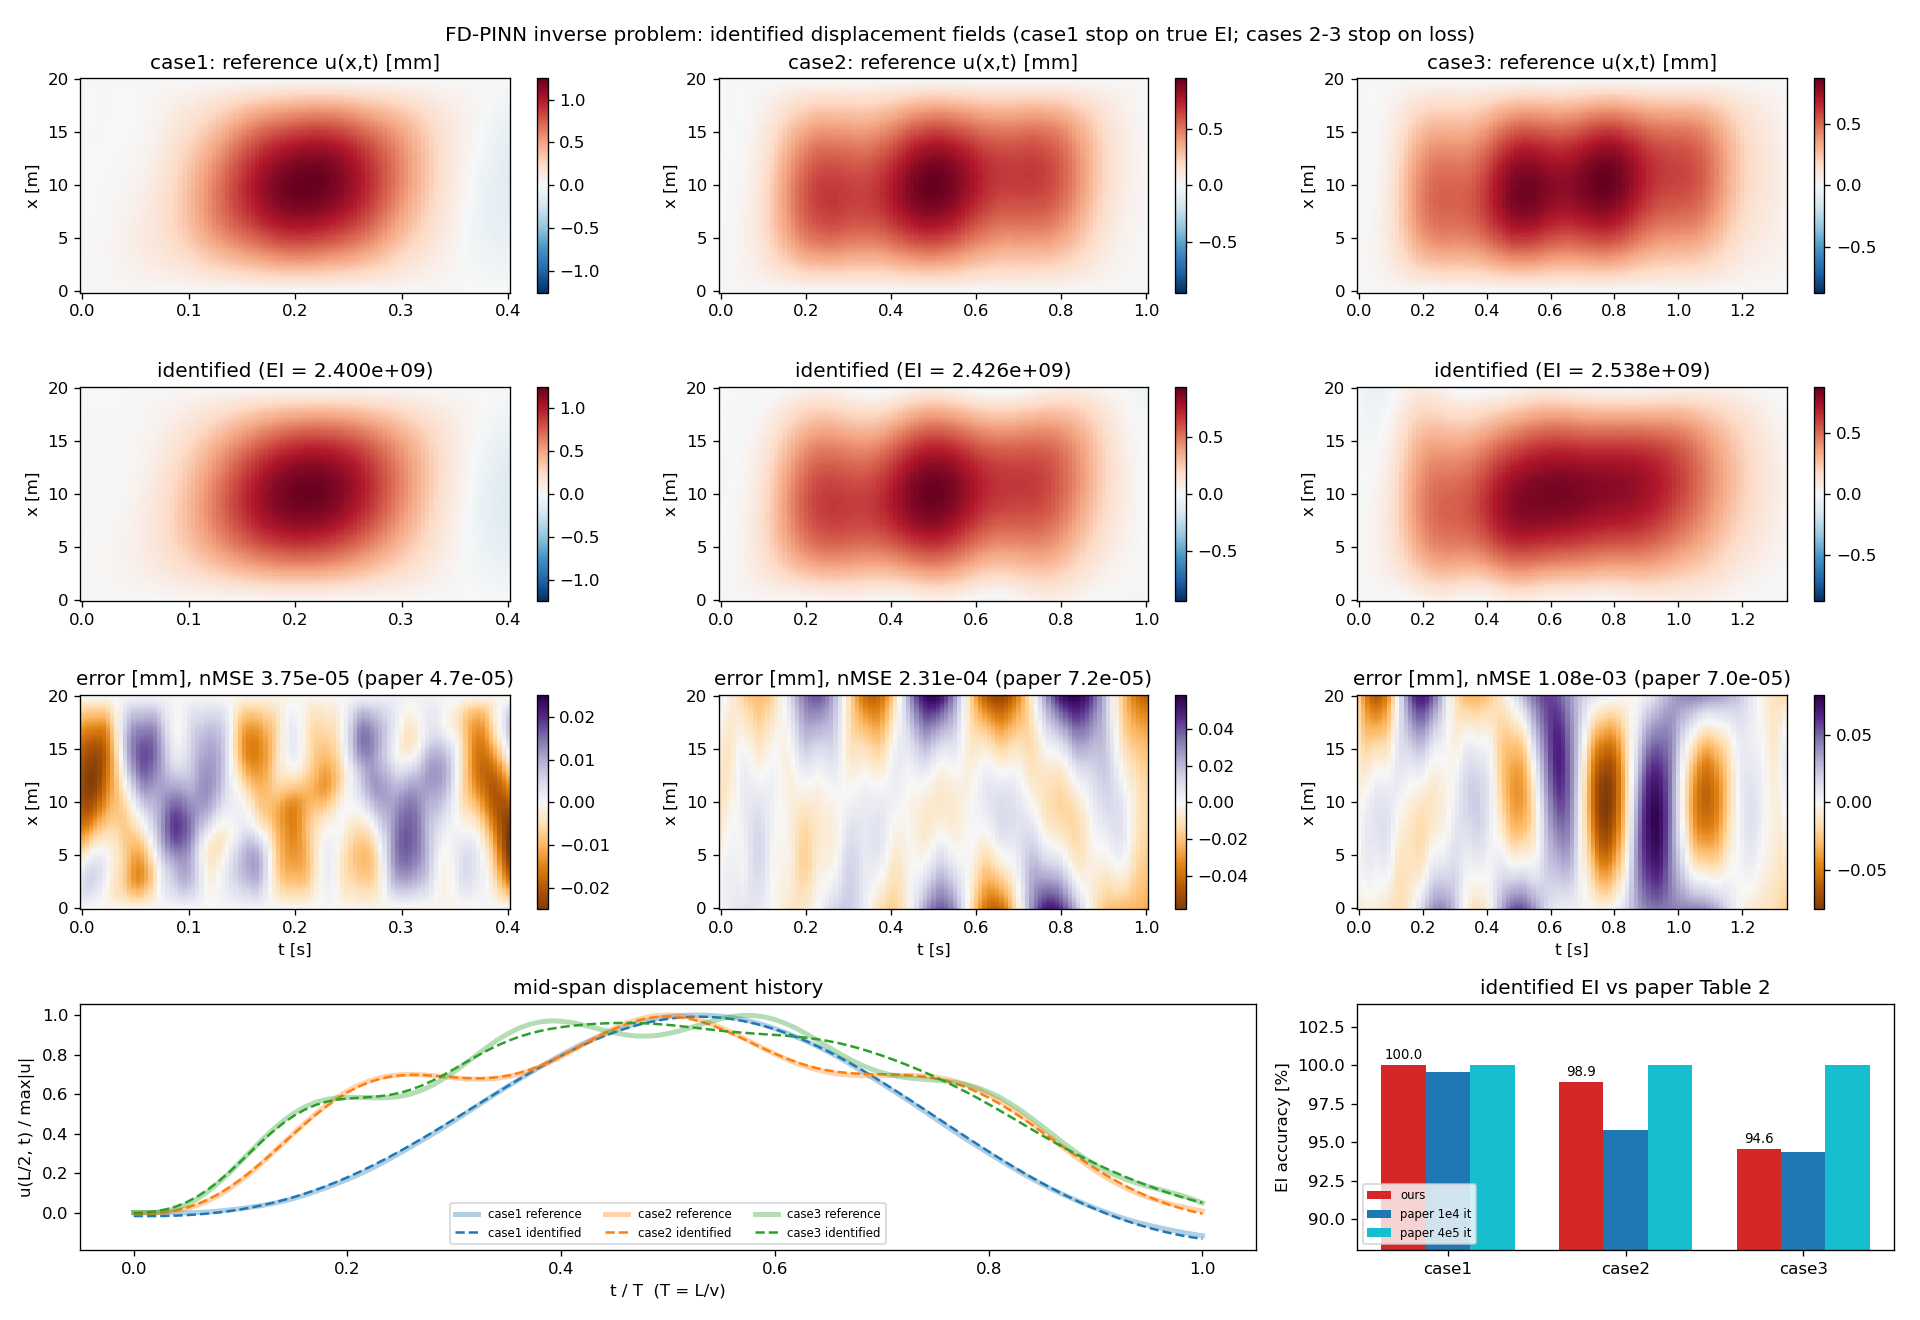
\includegraphics[width=0.95\linewidth]{figures/ch14r/fd_inv_fields.png}
\caption{Identified displacement fields, error maps, mid-span histories and accuracy against the publication, three cases. Plot of the reproduction report.}\label{fig:vf-fd-fields}
\end{figure}

\emph{The Case 3 bias.} None of four changes removed the $+5.7$ to $+7.4\,\%$ error of $EI$ (\Cref{tab:vf-fd-bias}), so it is not caused by float precision, the number of sensor frequencies, the number of collocation points or a wider band at this budget. The 0--8~Hz run is worse because it is under-trained ($\mathcal L_{DE}$ stayed near 650 against about 7 at 5~Hz), so it is confounded with the budget and says nothing about band choice at a larger budget. The 20\,000-point run is the cleanest negative result: the same plateau at $2.65$--$2.70\times10^9$ (about $89\,\%$) until iteration 7500, then a drift to $2.51$--$2.55\times10^9$, with the accuracy wandering between $93.6\,\%$ and $95.6\,\%$ over the last 6000 iterations while the loss keeps falling; the restored point was iteration 15\,000 ($94.63\,\%$), and the last point ($95.59\,\%$) was not selected because picking it would need the true $EI$. A 61\,000-iteration run to test whether the bias is under-training was aborted at about iteration 5000 with $EI$ at $2.68\times10^9$ ($89.6\,\%$), before the point where the baseline leaves its plateau, so that hypothesis is neither confirmed nor ruled out.

\begin{table}[tbp]
\centering\footnotesize
\caption{Case 3 (loss rule): runs tried against the $EI$ bias.}\label{tab:vf-fd-bias}
\begin{tabular}{@{}lrrrr@{}}
\toprule
Run & $EI$ identified & Error & Accuracy & Field nMSE\\
\midrule
Baseline (5000 points, 201 frequencies, 0--5 Hz, fp32) & $2.5382\times10^9$ & $+5.8\,\%$ & $94.56\,\%$ & $1.08\times10^{-3}$\\
Full 16\,000 iterations, no early stop & $2.5506\times10^9$ & $+6.3\,\%$ & $94.10\,\%$ & not stored\\
float64 & $2.5778\times10^9$ & $+7.4\,\%$ & $93.10\,\%$ & $1.01\times10^{-3}$\\
801 sensor frequencies & $2.5561\times10^9$ & $+6.5\,\%$ & $93.89\,\%$ & $1.12\times10^{-3}$\\
20\,000 collocation points & $2.5361\times10^9$ & $+5.7\,\%$ & $94.63\,\%$ & $9.85\times10^{-4}$\\
0--8 Hz band & $2.8660\times10^9$ & $+19.4\,\%$ & $83.74\,\%$ & $3.45\times10^{-3}$\\
\bottomrule
\end{tabular}
\end{table}

\begin{figure}[tbp]
\centering
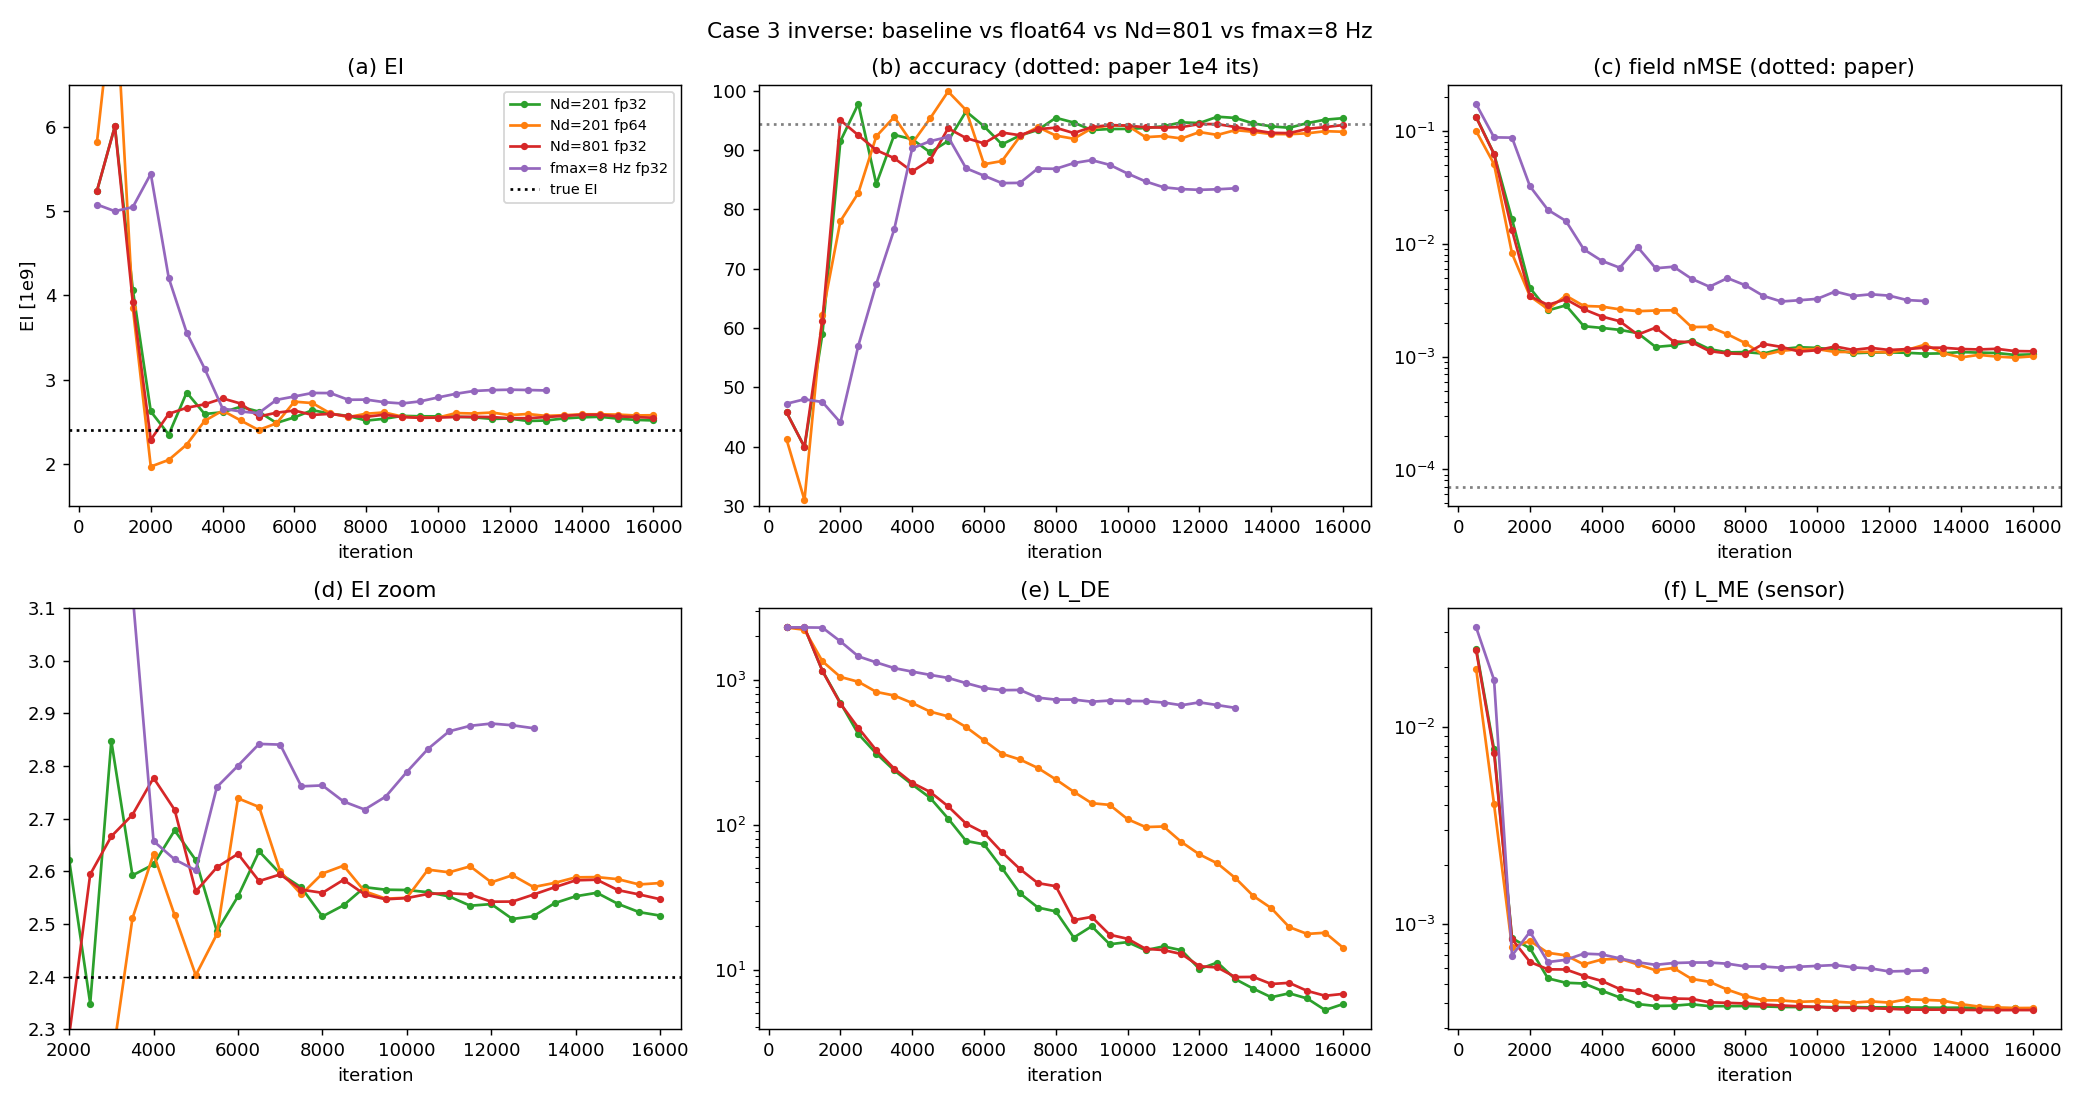
\includegraphics[width=0.95\linewidth]{figures/ch14r/fd_tests.png}
\caption{Case 3: $EI$, accuracy, nMSE and loss histories for the baseline, float64, 801-frequency and 0--8~Hz runs. Plot of the reproduction report.}\label{fig:vf-fd-tests}
\end{figure}

\subsection*{Why the results differ from the publication}

The three mismatches share one most likely cause, a training budget about 30 times smaller than the publication's, but only one explanation is verified by calculation; \Cref{tab:vf-fd-why} labels the status of each.

\begin{table}[tbp]
\centering\footnotesize
\caption{Explanations of the mismatches and their status.}\label{tab:vf-fd-why}
\begin{tabularx}{\linewidth}{@{}>{\raggedright\arraybackslash}p{4.2cm} >{\raggedright\arraybackslash}X >{\raggedright\arraybackslash}p{3.0cm}@{}}
\toprule
Mismatch & Most likely explanation & Status\\
\midrule
Case 3 inverse field nMSE $1.08\times10^{-3}$ against $7\times10^{-5}$ & mostly the $EI$ bias, not a separate failure & verified by calculation\\
Case 3 $EI$ stays $+5.7\,\%$ high & under-training of a sharp, low-amplitude resonance feature & supported; one test aborted\\
Forward FD-PINN $2.4\times10^{-3}$ against $7\times10^{-5}$ & 30 times fewer iterations, 4 times fewer points, no output transform & supported by training curves, not isolated\\
Time-domain PINN needed a source-width ramp & unknown implementation difference & hypothesis\\
Ranking of Cases 2 and 3 & Case 3 carries the least resonance content & hypothesis, consistent with the publication\\
\bottomrule
\end{tabularx}
\end{table}

\emph{The field error is mostly the $EI$ bias (verified).} A field that solves the equation exactly with the wrong $EI$ is already far from the reference. Solving Case 3 analytically at the identified $EI$, with the damping held at its true value as in the inverse runs, gives an nMSE of $8.4\times10^{-4}$ at the 20\,000-point value of $EI$ and $8.6\times10^{-4}$ at the baseline's, which is $85\,\%$ and $80\,\%$ of the measured network errors ($9.85\times10^{-4}$ and $1.08\times10^{-3}$). A $5.7\,\%$ rise in $EI$ raises $f_1$ by $2.8\,\%$ (\cref{eq:fd-f1}), which shifts the resonance ripple out of phase with the reference. The field error of an exact solution grows roughly with the square of the $EI$ error, so the publication's inverse MSE of $7\times10^{-5}$ corresponds to an $EI$ error of about $1.6\,\%$ (accuracy near $98.4\,\%$); at $94.4\,\%$ the same calculation gives about $9\times10^{-4}$. The publication's inverse MSE most likely comes from a later, more accurate iterate than its $10^4$-iteration accuracy; the notes do not say which. The network does slightly better or worse than the exact solution at the same $EI$, and the exact solution at the biased $EI$ keeps the double hump while the network smooths it out, which is the spectral bias the publication describes (\Cref{fig:vf-fd-bias}).

\begin{figure}[tbp]
\centering
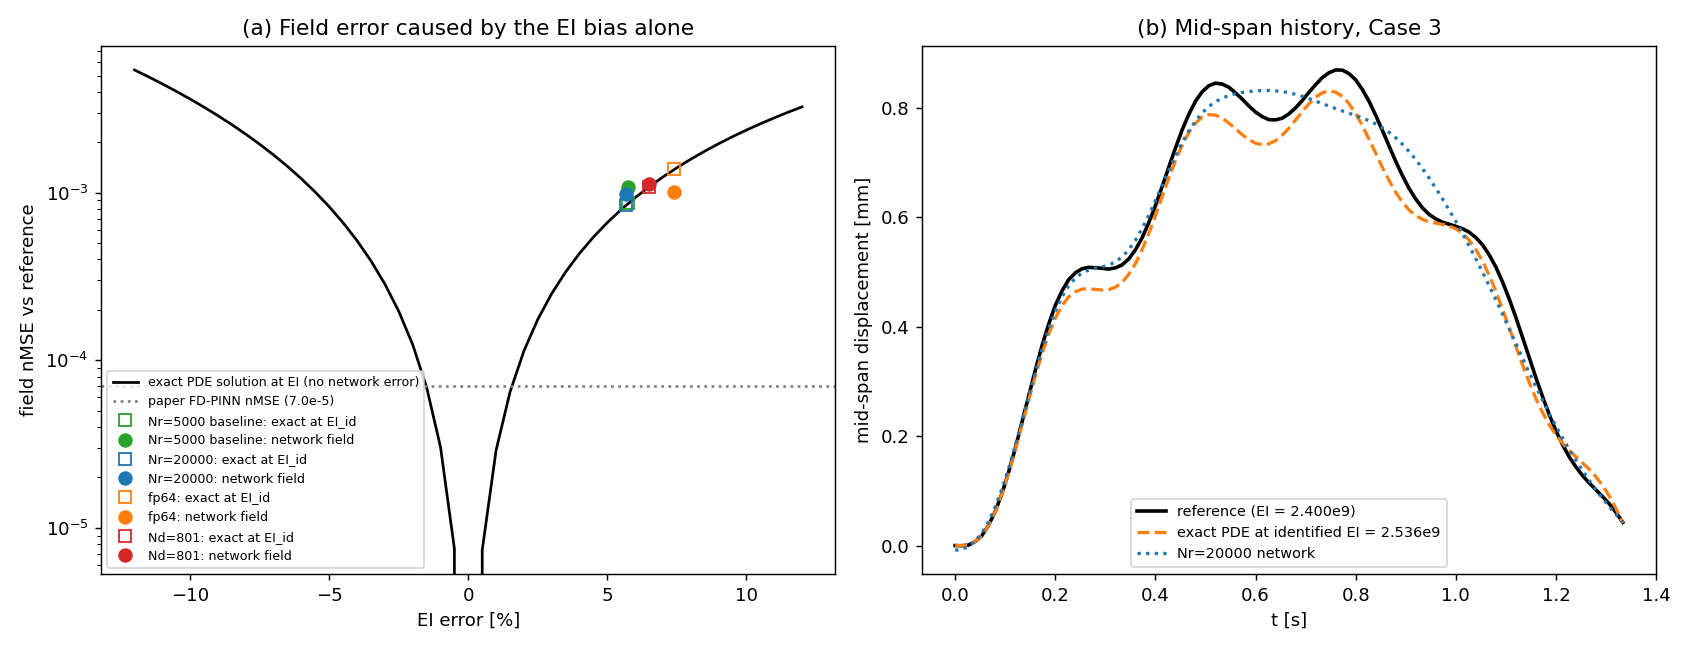
\includegraphics[width=0.95\linewidth]{figures/ch14r/fd_bias.png}
\caption{Left: field nMSE of an exact solution against the $EI$ error with the runs overlaid (squares: exact solution at the identified $EI$; circles: network field). Right: Case 3 mid-span history of the reference, the exact solution at the identified $EI$ and the network. Plot of the reproduction report.}\label{fig:vf-fd-bias}
\end{figure}

\emph{Why Case 3 is the hardest (supported).} The load's own frequency is $v/2L$: $1.25$, $0.5$ and $0.375$~Hz, so $f_1$ is $2.8$, $7.0$ and $9.4$ times the load frequency. In Case 1 the beam is driven much closer to resonance and the response is mostly the large resonance term; in Case 3 it is mostly a quasi-static lobe with a small resonance ripple, which a $3\times60$ network must resolve along $\omega$ in a peak $3.5\,\%$ of the band wide while the rest of the spectrum is smooth. A network that cannot represent the ripple can absorb part of the misfit by moving $EI$, so both the residual and the sensor misfit are small at a biased $EI$: the loss keeps falling ($\mathcal L_{DE}$ from $2.3\times10^3$ to 4) but the misfit term is flat at about $3.7\times10^{-4}$. This is a hypothesis for the ordering and not a measured result; both the publication ($99.6$, $95.8$, $94.4\,\%$ at $10^4$ iterations) and this work ($100$, $98.9$, $94.6\,\%$) rank Case 1 first and Case 3 last.

\emph{Forward accuracy (supported).} The error against the band-limited reference is $2.37\times10^{-3}$, so the formulation and the band are not the limit ($4\times10^{-6}$); the residual loss was still falling after the restored iteration while the nMSE crept up, and the long plateau followed by sudden drops is typical of L-BFGS on a stiff PINN loss when the budget is short. The budget is 13\,000 iterations against $4\times10^5$, with 5000 collocation points against 20\,000 and no output transform; no single one was isolated. Single-precision L-BFGS (the NaN guard fired in several runs) and framework differences are plausible but unverified. For the time-domain PINN, the plain recipe is a known failure of PINNs with a narrow Gaussian source, because the zero solution has a small residual away from the load; the publication's code is stated as available only after publication, so initialisation, loss weights and the Dirac width cannot be compared, and the ratio of $2.5$ compares recipes as much as budgets.

\subsection*{Comparison with the publication}

\begin{table}[tbp]
\centering\footnotesize
\caption{Outcome of the reproduction of \citet{liang2024fdpinn}.}\label{tab:vf-fd-cmp}
\begin{tabularx}{\linewidth}{@{}>{\raggedright\arraybackslash}p{4.4cm} >{\raggedright\arraybackslash}X >{\raggedright\arraybackslash}p{2.6cm}@{}}
\toprule
Quantity & This work & Outcome\\
\midrule
Reference solutions & analytical, Newmark, modal agree to $\sim10^{-7}$; band cost $3.8\times10^{-5}$, $5.6\times10^{-6}$, $4.0\times10^{-6}$ & reproduced\\
Inverse accuracy, Cases 1--3 & $100.0$, $98.9$, $94.6\,\%$ against $99.6$, $95.8$, $94.4\,\%$ & reproduced at $10^4$ its\\
Inverse near-$100\,\%$ at $4\times10^5$ iterations & not run & not tested\\
Forward FD-PINN, Case 3 & $2.38\times10^{-3}$ against $7.0\times10^{-5}$ & not reproduced (34$\times$)\\
Time-domain PINN, Case 3 & $3.90\times10^{-3}$ against $1.56\times10^{-3}$ (with a source ramp) & not reproduced (2.5$\times$)\\
Inverse-run field error, Case 3 & $1.08\times10^{-3}$ against about $7\times10^{-5}$ & not reproduced (about 15$\times$)\\
\bottomrule
\end{tabularx}
\end{table}

\subsection*{What was not reproduced, and why}

Five parts of the publication remain unchecked. The appendix beams B1--B3 have reference solutions, but FD-PINN has not been run on them. Only Case 3 was run forward. The long-budget test that would show whether the $EI$ bias disappears with training was aborted. At least three seeds per result are needed before differences of one or two accuracy points mean anything, because within one run the Case 3 accuracy moved between $93.6\,\%$ and $95.6\,\%$ over the last 6000 iterations; only the $19.4\,\%$ error of the 0--8~Hz run and the $5$--$7\,\%$ bias common to all runs exceed that spread. And noisy sensor data were not used, where the publication's inverse tests may include noise. The resonance hypothesis could be tested without further training by comparing the sensitivity of the sensor misfit to $EI$ in Cases 1 and 3.
